\documentclass[../main.tex]{subfiles}
\begin{document}

	В данном разделе введена модель трудоемкости алгоритмов. Посчитана сложность. Приведены схемы алгоритмов
	
\subsubsection{Оценка трудоемкости алгоритмов}

	Используется С-подобная модель оценки трудоемкости.
	
	Трудоемкость операций:
	\begin{enumerate}[1)]
		\item трудоемкость операций: \textbf{+, −, =, + =, − =, <, > ==, ++} равна 1;
		\item трудоемкость операций: *, /, \% равна 2;
		\item трудоемкость операции доступа к элементу памяти: [...] равна 3.
	\end{enumerate}

	Трудоемкость смены ячеек памяти местами будем считать 9, так как производится 3 обращения к памяти.
	
	Цикл будет оцениваться о фактически выполненным операциям из перечня выше.
	
	Условный оператор if будет фактически оценен как сумма стоимости операций в условии и трудоемкости различных ветвей (в лучшем случае и в худшем случае). 
	Стоимость условного перехода из уловия в одну из ветвей решения полагается равной 0.
	
\subsubsection{Классический алгоритм умножения матриц}

	Умножаются 2 матрицы M1(M, N), M2(N, Q). Ниже приведена формула рассчета сложности в в соответствии с моделью оценки трудоемкости.
	
	Итоговая формула: \\

	\begin{equation}
	\boxed{\begin{aligned}
		O(M, N, Q) = 8 * M * N * Q + 4 * M * N + 4 * M + 2
	\end{aligned}}
	\end{equation}

\subsubsection{Алгоритм Винограда}
	
	Умножаются 2 матрицы M1(M, N), M2(N, Q)
	
	\begin{enumerate}[1)]
		
		\item цикл 1: 
		\begin{equation}
		\label{eq:4}
		\boxed{\begin{aligned}
			2 + M(2 + 3 + \frac{N}{2} * (3 + 10))
		\end{aligned}}
		\end{equation}
		
		\item цикл 2:
		\begin{equation}
		\label{eq:5}
		\boxed{\begin{aligned}
			2 + Q(2 + 3 + \frac{N}{2} * (3 + 10))
		\end{aligned}}
		\end{equation}
		
		\item цикл 3:
		\begin{equation}
		\label{eq:6}
		\boxed{\begin{aligned}
			2 + M(2 + 2 + Q(2 + 7 + 3 + \frac{N}{2} * (3 + 20)))
			\end{aligned}}
		\end{equation}
		
	\end{enumerate}

	Условие четности/нечетности:
	
	\begin{equation}
	\label{eq:7}
	\boxed{\begin{aligned}
 	 1 + \begin{cases}
 	 	2 + M(2 + 2 + Q(2 + 10)), \textbf{N нечетное (худший вариант)} \\
 	 	0, \textbf{ иначе (лучший вариант)}
 	 \end{cases}
	\end{aligned}}
	\end{equation}
	
	Итоговая формула получается из суммы \ref{eq:4}, \ref{eq:5}, \ref{eq:6}, \ref{eq:7}
	
\subsubsection{Оптимизированный алгоритм Винограда}

	Умножаются 2 матрицы M1(M, N), M2(N, Q)
	
	\begin{enumerate}[1)]
		
		\item цикл 1:
		\begin{equation}
		\label{eq:8}
		\boxed{\begin{aligned}
			2 + M(2 + 2 + d(2 + 10))
			\end{aligned}}
		\end{equation}
		
		\item цикл 2:
		\begin{equation}
		\label{eq:9}
		\boxed{\begin{aligned}
			2 + Q(2 + 2 + d(2 + 10))
			\end{aligned}}
		\end{equation}
		
		\item цикл 3:
		\begin{equation}
		\label{eq:10}
		\boxed{\begin{aligned}
			2 + M(2 + 2 +Q(2 + 5+ 2 + d(2 + 20)))
			\end{aligned}}
		\end{equation}
		
	\end{enumerate}

	Условие четности/нечетности:

	\begin{equation}
	\label{eq:11}
	\boxed{\begin{aligned}
		1 + \begin{cases}
		2 + M(2 + 2 + Q(2 + 10)), \textbf{N нечетное (худший вариант)} \\
		0, \textbf{ иначе (лучший вариант)}
		\end{cases}
		\end{aligned}}
	\end{equation}
	
	Итоговая формула получается из суммы \ref{eq:8}, \ref{eq:9}, \ref{eq:10}, \ref{eq:11}
	
\subsection{Схемы}

	В данном подразделе приведены следующие схемы:
	\begin{enumerate}[1)]
		\item Cхема распараллеливания \ref{fig:parallel-function};
		\item Распараллеленный алгоритм Винограда \ref{fig:winiger1}, \ref{fig:winiger2}.
	\end{enumerate}
	
	\begin{figure}[H]
		\centering
		\includegraphics[scale=0.3]{"img/parallel function"}
		\caption[Схема функции распаралеливания]{Схема функции распаралеливания}
		\label{fig:parallel-function}
	\end{figure}
	
	\begin{figure}[H]
		\centering
		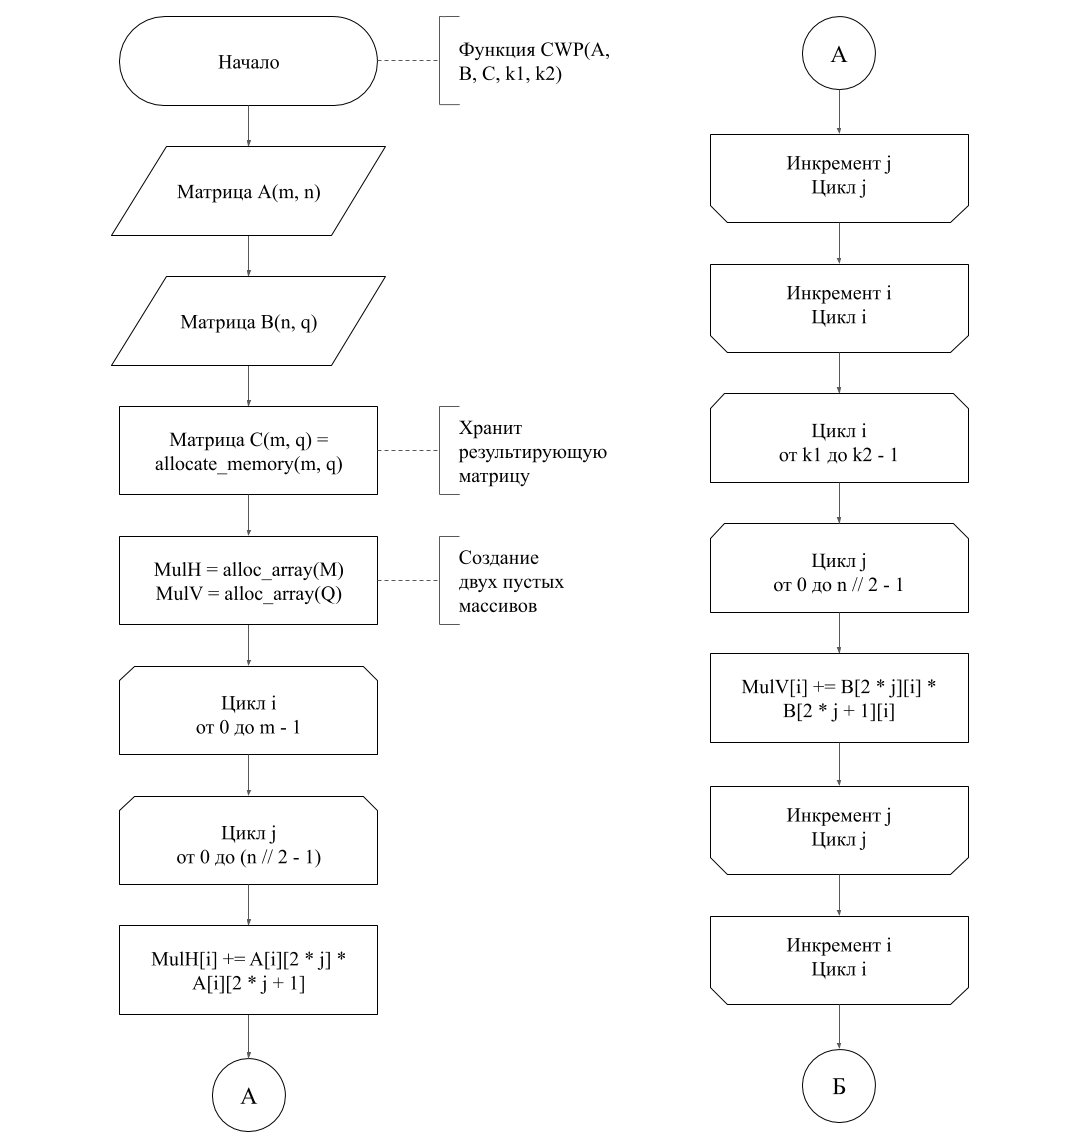
\includegraphics[scale=0.5]{img/Winiger1}
		\caption[Распараллеленный алгоритм Винограда. Часть 1]{Распараллеленный алгоритм Винограда. Часть 1}
		\label{fig:winiger1}
	\end{figure}

	\begin{figure}[H]
		\centering
		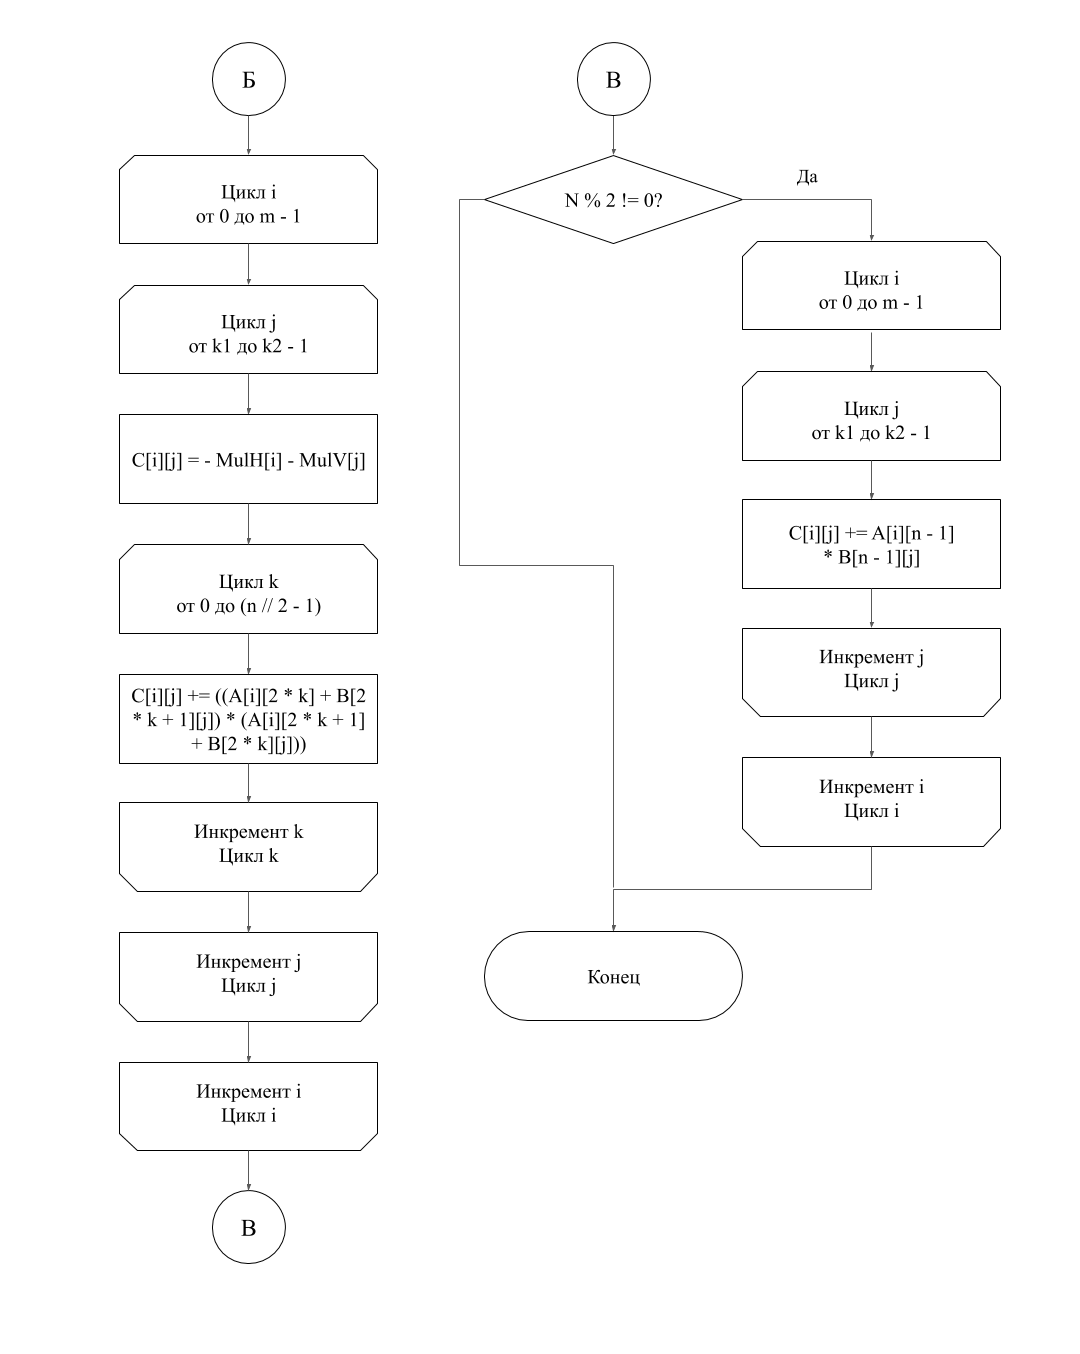
\includegraphics[scale=0.5]{img/Winiger2}
		\caption[Распараллеленный алгоритм Винограда. Часть 2]{Распараллеленный алгоритм Винограда. Часть 2}
		\label{fig:winiger2}
	\end{figure}
	
\subsection{Вывод}
	
	В данном разделе была введена модель трудоемкости. Вычислена трудоемкость каждого алгоритма. Указаны схемы алгоритмов.

\end{document}